\chapter{Testing}

Testing methodologies are used to ensure about the reliability, correctness, functionality and quality of the Federated Learning Web Console.
 In this chapter, the testing methodologies used in the project are described. The testing methodologies are divided into two main categories: structural testing and functional testing.

\section{Structural Testing}

%The structural testing performed on the project is described in this section.
Structural testing, also known as white-box testing is applied to the project to ensure that the implemented code is working as expected and evaluate the internal structure of the system.
For primary structure testing JUnit testing is applied as a testing methodology.

\subsection{JUnit Testing}

The JUnit testing performed on the project of FL Web Console. The JUnit testing is applied to various classes like DAOs and Services to check whether the implemented code is working as expected or not and specified
requirement are hold by the methods. Some examples of the JUnit testing that performed on the classes:

\subsubsection{UserDAO}
The UserDAO class is an important component of the project which is responsible for interacting with the database to handle data related with users. With the help of the JUnit tests
different scenarios are tested to ensure that the implemented code is working as expected and the requirements are fulfilled. This scenarios are including creating new user, deleting existing user, finding user by some criterias.
These tests show the correctness of the CRUD operations of the UserDAO class. Below it can be seen an example of performing JUnit test for some methods in the UserDAO.

\begin{figure}[ht!]
    \centering
    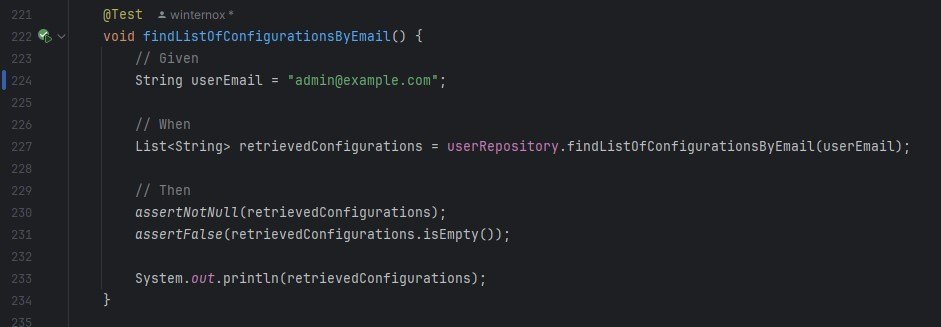
\includegraphics[width=0.8\textwidth]{images/5_testing/userdao-test}
    \caption{Testing the method of findListOfConfigurationsByEmail() in UserDAO class}
    \label{fig:u_dao_test}
\end{figure}

\begin{figure}[ht!]
    \centering
    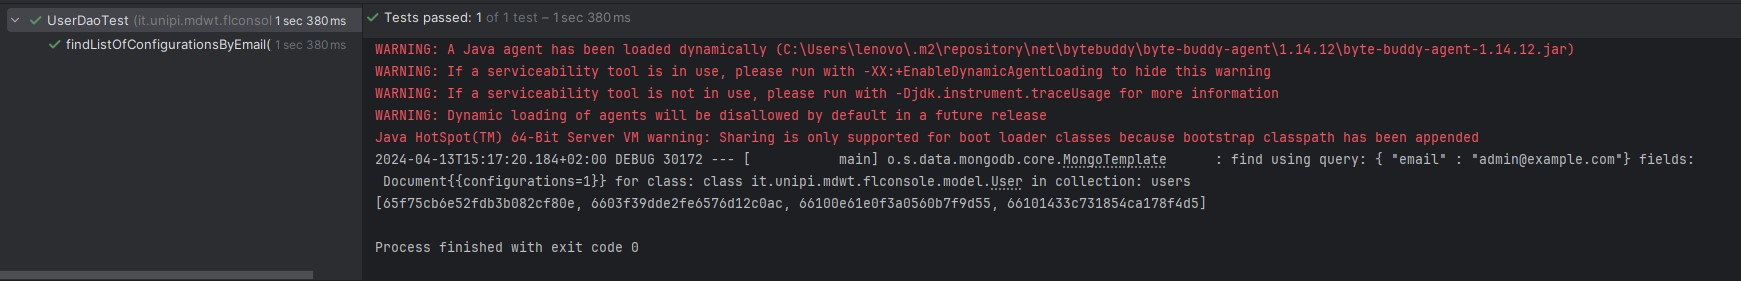
\includegraphics[width=0.8\textwidth]{images/5_testing/userdao-test-result}
    \caption{Testing result for the method of findListOfConfigurationsByEmail() in UserDAO class}
    \label{fig:u_dao_test_result}
\end{figure}

With this JUnit test method, the findListOfConfigurationsByEmail() method of the UserDAO class is tested. The test is performed by finding all the related configuration that are belong to the user with that email.
The test is successful and the expected result is returned as a list of configurations.

\newpage
\subsubsection{ExperimentDAO}
Experiment DAO is another important class of the project which is responsible for interacting with the database to handle data related with experiments. JUnit tests are created to ensure that the experiment related functions are
working as expected and the requirements are fulfilled. The tests are including creating new experiment, updating existing experiment, deleting existing experiment, finding experiment by some criterias. Below it can be seen an example test method for update an experiment.

\begin{figure}[ht!]
    \centering
    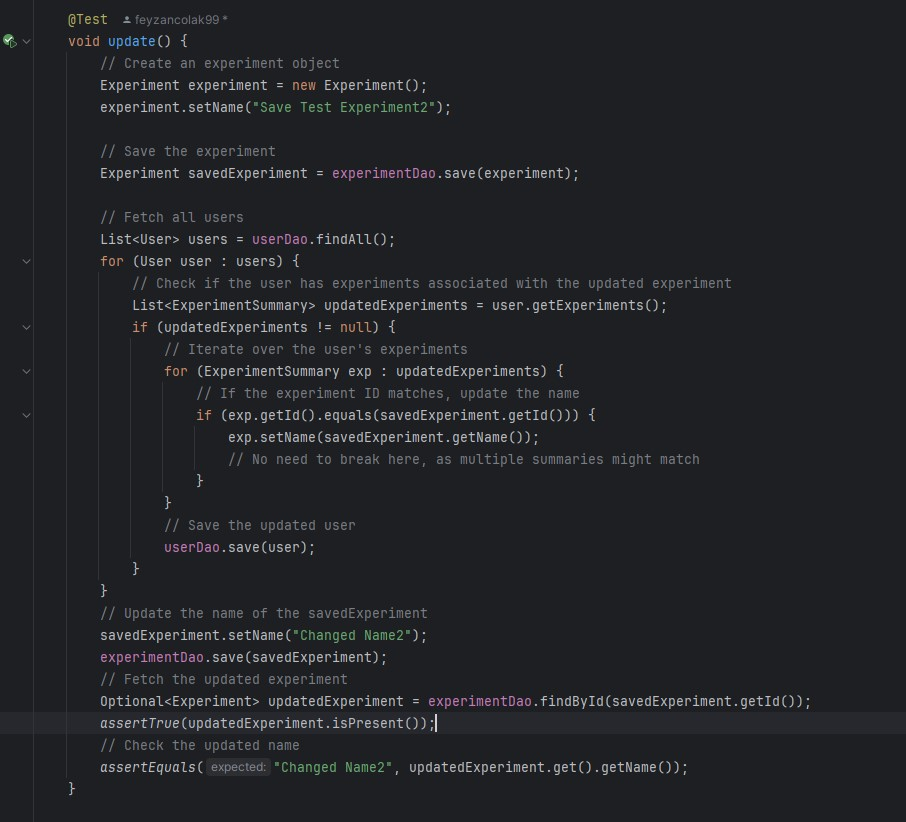
\includegraphics[width=0.8\textwidth]{images/5_testing/experimentdao-test}
    \caption{Testing the method of update() in ExperimentDAO class}
    \label{fig:e_dao_test}
\end{figure}

\newpage
\subsubsection{ConfigurationDAO}

Test class for Configuration DAO is another example of JUnit test that is performed on the project. The Configuration DAO class is responsible for interacting with the database to handle storage and retrival of the system experiment configuration.
Implementing JUnit for this class guarantees that system operates the data in an intended way for configuration class. Below there is an example test and test result for saveAndRetrieve() method of Configuration DAO class. The test is performed by
saving a configuration and then retrieving it from the database. The test is successful and the expected result is returned.

\begin{figure}[ht!]
    \centering
    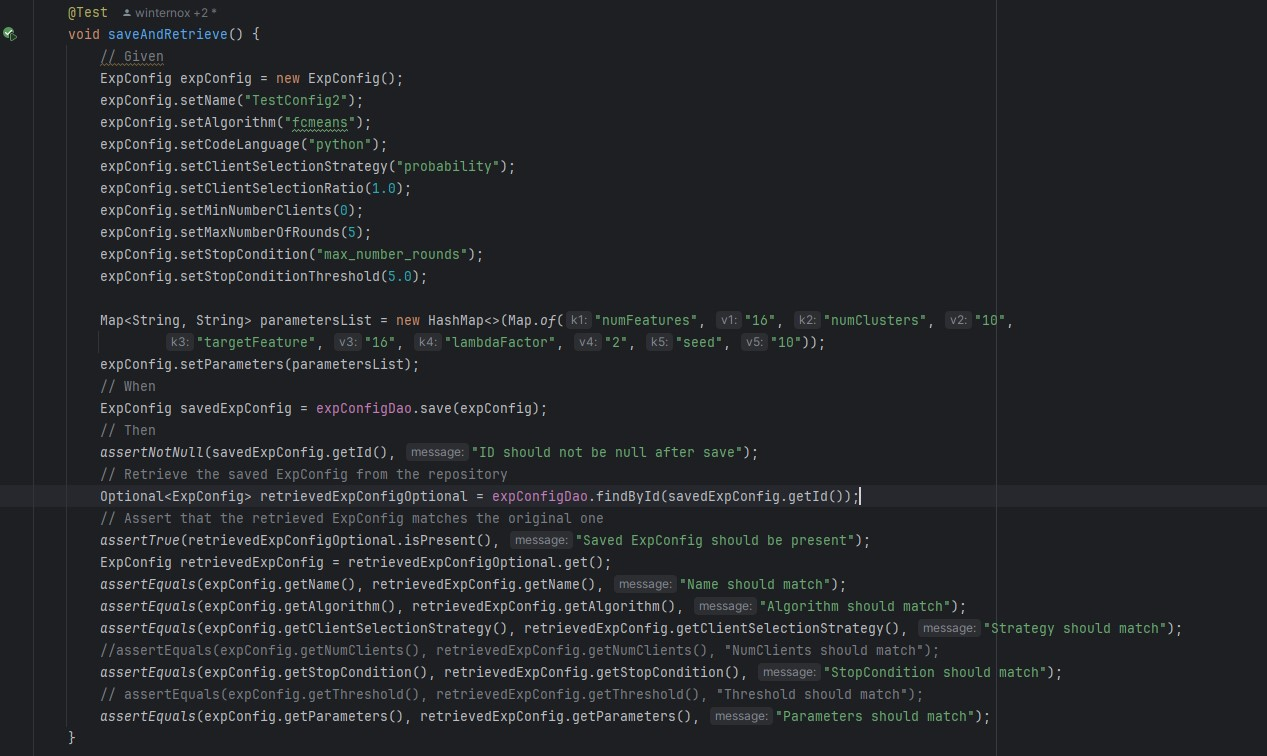
\includegraphics[width=0.8\textwidth]{images/5_testing/expconfigdao-test}
    \caption{Testing the method of saveAndRetrieve() in Configuration DAO class}
    \label{fig:c_dao_test}
\end{figure}

\begin{figure}[ht!]
    \centering
    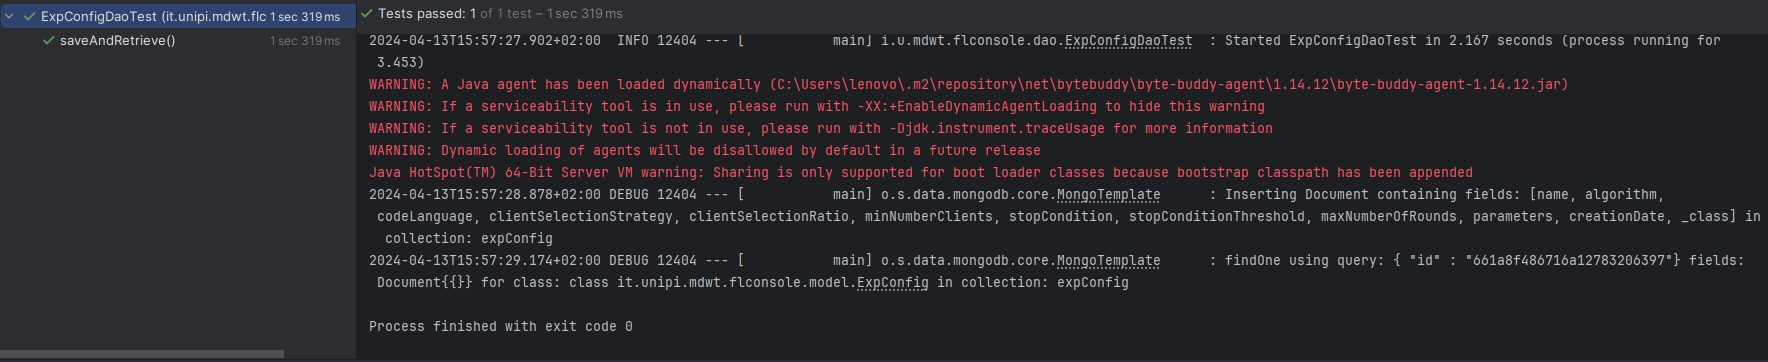
\includegraphics[width=0.8\textwidth]{images/5_testing/expconfigdao-test-result}
    \caption{Testing result for the method of saveAndRetrieve() in Configuration DAO class}
    \label{fig:c_dao_test_result}
\end{figure}


\newpage
\section{Functional Testing}

%The functional testing performed on the project is described in this section.
Functional testing, also known as black-box testing is applied to the project to evaluate the system behaviour that needs to fulfill functional requirements.
Functional testing helps to ensure that user expectations are provided in a right way. The functional testing is performed by creating test cases for the system.\\

Test cases are identified according to the functional requirements. It shows how the system should behave in different scenarios that are both normal and anormal.
Those test cases are including user authentication, creating new configuration, creating new experiment, deleting experiment, finding experiment, finding configuration, deleting configuration, etc.
Below there is a table that shows some examples of the test cases that are created for the project. As a result of the test cases, it can be said that the Federated Learning Web Console provides all the
necessary functionalities and meets user expectations.

\subsection{Test Cases}

%\begin{table}[ht!]
%    \centering
%    \caption{Test case}
%    \begin{tabularx}{\textwidth}{|Sl|S{X}|S{X}|S{X}|S{X}|S{X}|}
%        \hline
%        \textbf{Id} & \textbf{Description} & \textbf{Input} & \textbf{E. Output} & \textbf{Output} & \textbf{Outcome} \\ \hline
%        U\_T\_01    & Lorem Ipsum          & Lorem Ipsum    & Lorem Ipsum         & Lorem Ipsum     & Lorem Ipsum      \\ \hline
%        U\_T\_02    & Lorem Ipsum          & Lorem Ipsum    & Lorem Ipsum         & Lorem Ipsum     & Lorem Ipsum      \\ \hline
%        U\_T\_03    & Lorem Ipsum          & Lorem Ipsum    & Lorem Ipsum         & Lorem Ipsum     & Lorem Ipsum      \\ \hline
%        U\_T\_04    & Lorem Ipsum          & Lorem Ipsum    & Lorem Ipsum         & Lorem Ipsum     & Lorem Ipsum      \\ \hline
%        U\_T\_05    & Lorem Ipsum          & Lorem Ipsum    & Lorem Ipsum         & Lorem Ipsum     & Lorem Ipsum      \\ \hline
%    \end{tabularx}
%\end{table}

\begin{table}[ht!]
    \centering
    \caption{Test case}
    \begin{tabularx}{\textwidth}{|Sl|S{X}|S{X}|S{X}|S{X}|S{X}|}
        \hline
        \textbf{Id} & \textbf{Description} &            \textbf{Input} &                        \textbf{E. Output} &                            \textbf{Output} &                       \textbf{Outcome} \\ \hline
        U\_T\_01    & User Authentication               & Email:admin@example.com                & Login Successfully and                       & Redirected to admin dashboard          & Passed     \\ \hline
                                                          password: Adm1nP@ss
                                                          (valid credentials)
        U\_T\_02    & User Authentication 2             & Email: invalid@example.com             & Error message displayes                      & Unable to login                        & Passed    \\ \hline
                                                            password: invalid
                                                            (invalid credentials)
        U\_T\_03    & Creating New Configuration        & Adding all the necessary values to     & Configuration Created successfuly            & Configuration Created successfuly      & Passed     \\ \hline
                                                            the new FL configuration form
        U\_T\_04    & Creating New Configuration 2      & Entering all the values                & Error of missing value message is displayed  & Configuration is not created           & Passed       \\ \hline
                                                            except stop condition
        U\_T\_05    & Creating New Experiment           & Name is written and FL                 & Experiment Created successfuly               & Experiment Created successfuly         & Passed     \\ \hline
                                                            configuration is selected
    \end{tabularx}
\end{table}
